\chapter{Introducción}

\section{Tecnologías de secuenciación en medicina de precisión}

Las secuencias genómicas determinan aspectos fundamentales de la biología de los 
organismos y proporcionan información sobre su historia evolutiva. La aplicación 
de este conocimiento genómico a la salud humana ha dado lugar a la medicina de 
precisión, una disciplina que aprovecha los marcadores genéticos y moleculares
para personalizar los tratamientos médicos según las características individuales 
de cada paciente \cite{collins_new_2015}. Los avances en las plataformas de secuenciación y las 
herramientas bioinformáticas estan permitiendo capturar variaciones genéticas, 
interpretar sus consecuencias funcionales y trasladar estos hallazgos a la práctica
clínica \cite{carrasco-ramiro_human_2017}.

Los métodos de secuenciación del ADN han evolucionado significativamente a lo 
largo de los años, desde un enfoque práctico podemos dividirlos en tres categorías 
principales:

\begin{itemize}
    
    \item \textbf{Método de terminación de cadena}: se basa en la terminación 
    controlada de la síntesis de ADN, generando fragmentos de diferentes 
    longitudes que revelan la secuencia al separarse por tamaño (\textbf{Figura~\ref{fig:sanger_seq}}). 
    Aunque su baja capacidad de paralelización la ha relegado frente a la 
    secuenciación masiva en proyectos genómicos, sigue siendo útil para verificar 
    secuencias cortas, como genes individuales amplificados por PCR \cite{moorcraft_understanding_2015}.

    \item \textbf{Secuenciación de lecturas cortas}: hace referencia al conjunto 
    de tecnologías que realizan secuenciación paralela y masiva de fragmentos de 
    ADN (250-600 bp) amplificados clonalmente (\textbf{Figura~\ref{fig:illumina_seq}}), 
    proporcionando gran profundidad de secuenciación y una precisión superior al 99,9\% 
    \cite{logsdon_long-read_2020}. La empresa Illumina domina mundialmente en esta 
    categoría, con MGI Tech como principal competidor emergente \cite{jeon_comparison_2021}.

    \item \textbf{Secuenciación de lecturas largas}: estas plataformas también
    emplean estrategias de secuenciación paralela, pero que generan lecturas 
    individuales que abarcan desde decenas hasta miles de kilobases. Dos métodos 
    principales dominan este campo: la secuenciación en tiempo real 
    de molécula única (SMRT, \textit{Single Molecule Real-Time}) 
    (\textbf{Figura~\ref{fig:long_seqs}A}), comercializada
    por PacBio, y mediante nanoporos, liderada por Oxford Nanopore Technologies 
    (ONT) (\textbf{Figura~\ref{fig:long_seqs}B}) y con la reciente aparición de una alternativa de MGI Tech 
    \cite{logsdon_long-read_2020,zhang_single-molecule_2024}.

\end{itemize}

\section{Contribución de las lecturas largas al análisis de variantes 
estructurales}

Las variantes genéticas se clasifican en tres categorías en base al número de 
nucleótidos alterados: variantes de un solo nucleótido (SNVs), pequeñas 
inserciones o deleciones (indels; 1-50 pb), y variantes estructurales (SVs; 
≥50 pb). Tanto SNVs como indels han sido ampliamente estudiadas debido a sus 
altas densidades mutacionales y relativa facilidad de detección mediante
plataformas de secuenciación y herramientas de análisis basadas en lecturas 
cortas \cite{collins_diversity_2025}. Pero estos enfoques son insuficientes para 
capturar la mayoría de SVs, particularmente aquellas que contienen secuencias 
altamente repetitivas o anomalías que abarquen grandes fragmentos cromosómicos, 
debido a la incapacidad inherente de las lecturas cortas para ser mapeadas 
correctamente a genomas humanos de referencia (\textbf{Figura~\ref{fig:fig_1}}) 
\cite{ho_structural_2020}.

\begin{figure}[H]
    \centering
    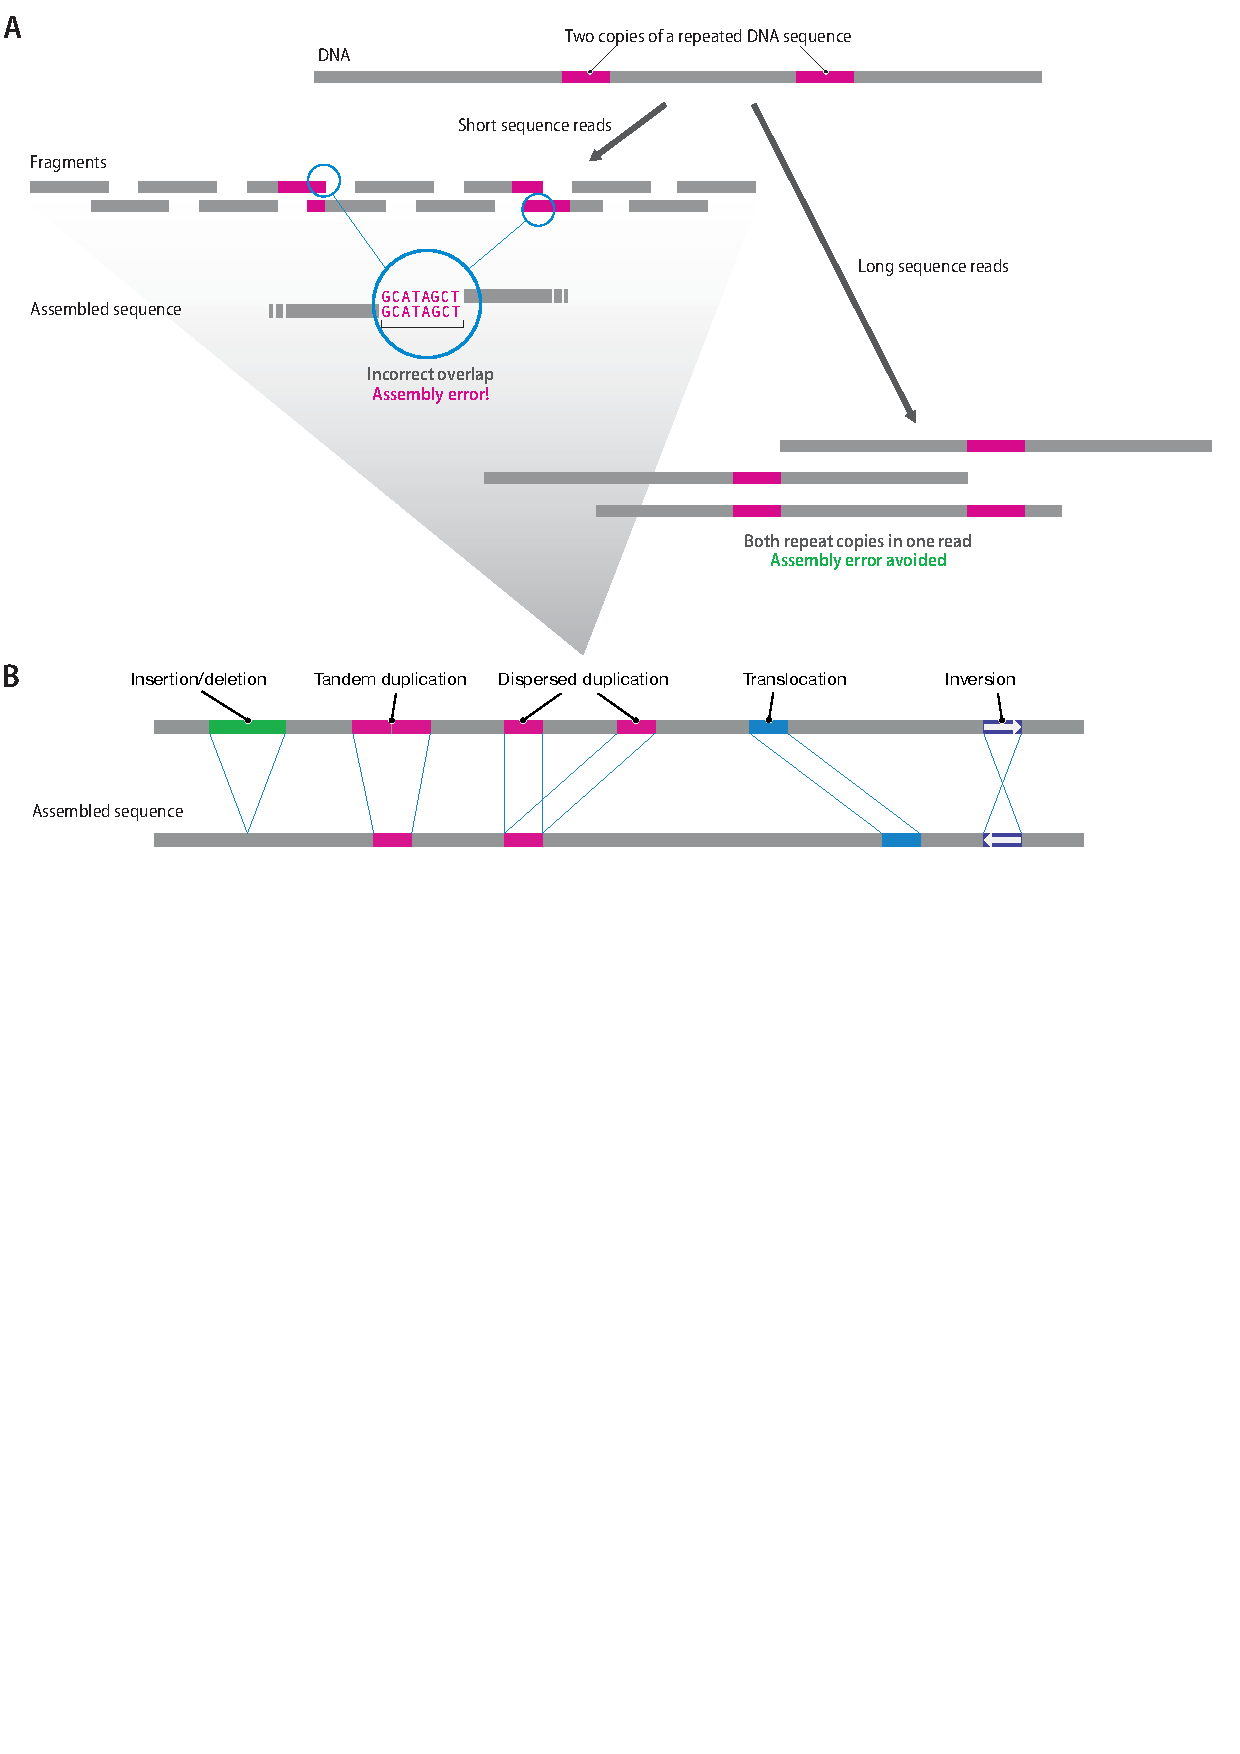
\includegraphics[width=\textwidth]{img/fig_1.pdf}
    \vspace{0.25cm}
    \caption[Limitaciones del ensamblaje genómico con lecturas cortas]{Limitaciones 
    del ensamblaje genómico con lecturas cortas. (\textbf{A}) Si una secuencia 
    contiene una duplicación dispersa de, por ejemplo, $\sim$500 pb y secuenciamos
    con lecturas cortas ($\sim$100 pb), herramientas de alineamiento pueden superponerlas 
    como una sola copia. Con lecturas largas ($\sim$10 kb), ambas copias se capturan 
    en una única lectura, resolviendo correctamente la duplicación. (\textbf{B}) 
    Esta dificultad se extiende a todos los tipos de SVs; inserciones, deleciones,
    duplicaciones, traslocaciones, inversiones o combinaciones de ellas. Adaptado
    de \cite{brown_genomes_2023}.}
    \label{fig:fig_1}
\end{figure}

Las tecnologías de secuenciación de lectura larga surgieron hace una década, 
marcando un punto de inflexión en el ensamblaje de secuencias al abordar las 
limitaciones de las lecturas cortas. Inicialmente, estas tecnologías tenían tasas 
de error mucho más elevadas ($\sim$10\%) en comparación con las lecturas cortas 
(< 1\%) \cite{espinosa_advancements_2024}. Si bien esto permitió el ensamblaje rutinario de genomas 
bacterianos, limitó su aplicación en genómica humana, particularmente para la 
detección de mutaciones puntuales \cite{loman_complete_2015}. Sin embargo, las 
mejoras continuas en las plataformas de secuenciación de lectura larga han reducido 
progresivamente estas tasas de error, permitiendo finalmente la generación del primer genoma de 
referencia humano sin huecos, conocido como ensamblaje telómero a telómero (T2T) 
\cite{nurk_complete_2022}. Este logro resolvió regiones genómicas previamente 
inaccesibles que permanecían incompletas en la versión 38 del genoma de referencia 
humano del Consorcio de Referencia Genómica (GRCh38) (ver \textbf{Figura \ref{fig:T2T_ref}}).

Más allá de las diferencias metodológicas de secuenciación, existen disparidades 
significativas entre las plataformas de lectura larga en términos de 
accesibilidad y coste. Aunque PacBio fue pionera en este campo en 2011 con 
sistemas de secuenciación de alto rendimiento, sus plataformas han requerido 
consistentemente inversiones de cientos de miles de dólares. En contraste, el 
lanzamiento del MinION por parte de ONT en 2014 supuso un cambio de paradigma al 
introducir un dispositivo portátil de bajo rendimiento con una inversión de 
apenas unos pocos miles de dólares \cite{espinosa_advancements_2024,noauthor_vega_nodate}. 

Posteriormente, ONT amplió su catálogo hacia la gama de alto rendimiento con los 
dispositivos PromethION, cuyo modelo de entrada ``P2 solo'' permite la secuenciación 
de genomas completos (WGS) mediante conexión a ordenador por menos de 20.000 
dólares. Esto ha hecho que la secuenciación de lectura larga sea económicamente 
accesible para la mayoría de laboratorios de biología molecular, desplazando el 
principal obstáculo hacia la formación especializada en bioinformática necesaria 
para el procesamiento y análisis de los datos generados \cite{oxford_nanopore_technologies_nanopore_nodate}.

La tecnología de secuenciación de ONT funciona mediante la medición de cambios 
en la corriente iónica a medida que moléculas individuales de ADN o ARN son 
translocadas por una enzima de desenrollamiento anclada a la superficie del 
nanoporo. Estos nanoporos están dispuestos en arrays sobre una celda de flujo
(\textit{flowcell}), el componente consumible fundamental de ONT, que alberga 
miles de canales de detección independientes. Los cambios individuales de corriente 
en cada nanoporo se interpretan mediante un modelo basado en redes neuronales 
entrenado con secuencias nucleotídicas sintéticas de contenido conocido y sus 
correspondientes variaciones de corriente, permitiendo determinar la secuencia 
de cada molécula que atraviesa el nanoporo (\textit{basecalling}) \cite{mardis_tracing_2025}.

Las mejoras recientes en la arquitectura de los nanoporos de las celdas de flujo 
(con la transición de la proteína de poro R9, con constricción de 9 Å, a la 
variante R10 que incorpora un barril elongado y constricción de 10 Å) y de los 
algoritmos de basecalling han mejorado significativamente la precisión de esta
técnica de secuenciación (\textbf{Figura~\ref{fig:ont_pores}}). Esto hace de la 
secuenciación por nanoporos un enfoque viable para el análisis sistemático de 
variantes asociadas a cáncer; incluyendo la reconstrucción de SVs, modificaciones
epigenéticas como metilaciones sin tratamientos adicionales como la conversión
por bisulfito, así como la asignación directa de estas variantes a sus respectivos 
cromosomas parentales (\textit{haplotype phasing}) 
\cite{kolmogorov_scalable_2023,sakamoto_phasing_2022,schaal_migrating_2022}.

\section{Variación estructural en cáncer}

Según el Instituto Nacional del Cáncer (NCI), el cáncer comprende más de 100 tipos 
diferentes que se originan cuando células normales experimentan alteraciones 
genéticas y/o epigenéticas que resultan en proliferación descontrolada y 
la alteración de la homeostasis del organismo \cite{noauthor_what_2007,hanahan_hallmarks_2011}. 
El desarrollo tumoral representa un proceso complejo producto de las interacciones entre el 
genotipo individual y diversos factores ambientales, impulsando una evolución 
clonal en la que diferentes subpoblaciones de células malignas compiten por 
recursos y espacio \cite{turajlic_resolving_2019}. La secuenciación del ADN 
tumoral permite la identificación de mutaciones \textit{driver} específicas de 
cada paciente, facilitando la selección e implementación más efectiva de terapias 
dirigidas \cite{sicklick_molecular_2019}.

La importancia de las variantes estructurales (SVs) como \textit{hallmark} del 
cáncer es cada vez más evidente. Un análisis reciente de 2.658 genomas tumorales 
reveló que aproximadamente el 50\% de las mutaciones \textit{driver} se solapan con 
SVs, destacando su papel crucial en el desarrollo del cáncer 
\cite{li_patterns_2020,menghi_tandem_2018}. A pesar de su importancia como 
biomarcadores en enfermedades oncológicas, nuestro conocimiento sobre las SVs sigue siendo limitado en comparación con las variantes 
de nucleótido único (SNVs). Esta brecha de conocimiento se debe principalmente a 
las limitaciones técnicas de la secuenciación de lectura corta, que ha dominado 
los proyectos de secuenciación genómica a gran escala. Utilizando lecturas cortas, 
la detección de SVs se basa principalmente en estimaciones de variaciones en el 
número de copias (CNVs), una medida indirecta que no logra capturar eventos 
como inversiones o translocaciones balanceadas 
\cite{cameron_comprehensive_2019,abel_mapping_2020}.

El equipo de investigación en secuenciación por nanoporos de la Unidad de 
Bioinformática del Centro Nacional de Investigaciones Oncológicas desarrolla, 
entre sus líneas prioritarias, análisis de genomas completos de pacientes con 
mieloma múltiple (MM) en estadios pre y post-tratamiento \cite{haertle_multi-omic_2026}. 
El MM es una neoplasia de células B terminalmente diferenciadas (células plasmáticas) 
caracterizada por translocaciones cromosómicas frecuentes que sitúan oncogenes 
bajo el control de potenciadores de expresión de inmunoglobulinas, así como por 
la adquisición de otras SVs de gran tamaño. Algunas de estas alteraciones, 
descritas por primera vez hace más de dos décadas, siguen siendo los 
principales marcadores pronósticos y son detectadas principalmente mediante 
hibridación fluorescente in situ (FISH) \cite{kuehl_multiple_2002}.

El MM sigue un patrón característico de remisión-recaída donde las células 
malignas adquieren progresivamente resistencia a múltiples líneas terapéuticas 
(\textbf{Figura~\ref{fig:evo_MM}}) \cite{kurtin_relapsed_2013}. En este contexto, la secuenciación por 
nanoporos de ONT junto con métodos automatizados de llamada de SVs podría ampliar 
nuestra comprensión de los mecanismos fisiopatológicos e identificar potencialmente 
nuevos marcadores pronósticos y objetivos terapéuticos, contribuyendo en última 
instancia a mejorar el manejo clínico y el pronóstico de supervivencia. 

\begin{figure}[H]
    \centering
    \includegraphics[width=0.7\textwidth]{img/evo_MM.png}
\caption[Ciclo de remisión-recaída del mieloma múltiple]{Ciclo de 
    remisión-recaída del mieloma múltiple. Se caracteriza por 
    ciclos sucesivos de respuesta, remisión y recaída bajo tratamiento, 
    monitorizados mediante niveles de proteína M (anticuerpo anómalo 
    producido por células plasmáticas malignas). Las recaídas sucesivas 
    acumulan SVs que generan evolución clonal con respuestas progresivamente 
    más breves y superficiales. Cortesía de Álvaro Otero Sobrino, Hospital 12 de Octubre.}
    \label{fig:evo_MM}
\end{figure}

\section{Justificación del proyecto}

En la última guía de recomendaciones para la bioinformática en la práctica 
clínica publicada en \textit{Genome Medicine}, los autores reconocen el valor de 
la secuenciación de lecturas largas para la detección de SVs, aunque también 
señalan la necesidad de establecer estándares consensuados por la comunidad 
científica respecto a las herramientas de detección de CNVs y SVs. Sin embargo, 
la evaluación de estos métodos sigue siendo compleja debido principalmente a la 
ausencia de \textit{datasets} curados y abiertos \cite{lavrichenko_recommendations_2025}.

La generación de modelos celulares que incorporen de manera estable conjuntos 
de SVs requeriría la implementación de procedimientos experimentales complejos, 
con una considerable inversión de tiempo y recursos económicos. Por el contrario, 
la utilización de datos sintéticos constituye una alternativa económicamente 
viable que, además, presenta la ventaja de conocer a priori la verdad absoluta, 
facilitando así la validación y evaluación de los métodos desarrollados.

Los datos experimentales son esenciales para crear y mejorar métodos 
computacionales, cuyos resultados no solo proporcionan nuevos conocimientos, 
sino que también pueden servir como base para refinar futuros experimentos. No
obstante, los datos sintéticos pueden ayudar a catalizar este ciclo, generando información más 
rápidamente y con un menor consumo de recursos.